\documentclass[10pt,a4paper]{report}
\usepackage[utf8]{inputenc}
\usepackage[francais]{babel}
\usepackage{xcolor}
\usepackage{graphicx}
\usepackage{amsmath,amsfonts,amssymb}


\title{Rapport d'Analyse Syntaxique et Projet de Programmation}

\date{\today}

\author{Claude Cugerone, Bérénice Faltrept, Amélie Guémon, Marin Liebert}

\begin{document}

\maketitle

Nous avons implémentés deux analyseurs qui vont produire trois pages html, un script en javascript et une feuille de style css. les pages html correspondent à : 
\begin{enumerate}
	\item L'affichage du code C du fichier d'origine.
	\item La documentation produite en respectant des balises doxygen.
	\item le résultat du traitement du fichier latex proprement présenté.
\end{enumerate}

Nous avons aussi écrit un script simple vous permettant de compiler puis lancer nos analyseur latex et c sur nos fichiers de tests et ainsi de générer les fichiers formant le site web. \\

\section{Analyse de la partie C}

\subsection{coloration}
La coloration a été faite en premier, elle m'a donc permis de découvrir les code flex et bison utilisés. La seule difficulté à été que j'avais préalablement fait toute la coloration dans le document flex, mais qu'elle ne permettait pas certains traitements (reconnaissance des déclarations/définitions séparés des utilisation de fonctions par exemple). J'ai donc pris le temps de tout transférer dans la grammaire. 

\subsection{commentaires}
Il s'agit du seul traitement que j'ai laissé dans le flex. Il a nécessité d'ajouter des règles a l'analyse lexicale ainsi qu'un état pour traiter les commentaire sur plusieurs lignes. \newline
On s'assure que dans tous les commentaires, les symboles spéciaux du html ne seront pas interprétés. Nous faisons de même dans les éléments du code que nous recopions directement dans le fichier final et qui risqueraient de poser problème : les instructions préprocesseur et les chaînes de caractères.

\subsection{traitement préprocesseur}
Il n'existait pas dans l'analyse lexicale initiale, nous avons donc rajoutés la règle permettant de les acceptés. Comme pour les commentaires et la documentation, il s'agit d'un traitement qui aurait été coûteux si un tampon n'était pas intégré à \textit{fprintf}, car nous traitons chaque caractère séparément. 

\subsection{indentation}
	Un des critères de bonne lisibilité du code est l'indentation, que nous avons gérés avec une variable globales entière. Là ou nous avons eu des difficultés, ce fut pour traiter les blocs de conditions ne possédant pas d'accolade.
	\newline
	dans l'exemple qui suit, on voit qu'il faut insérer un saut de ligne et une indentation directement après la fin des parenthèses pour le if, mais après l'accolade pour le else. \newline
	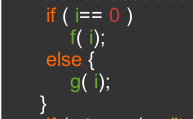
\includegraphics[height=2cm]{site/indent1.png} 
	\newline 
Pour cela, j'avais besoin dans la grammaire, d'accéder au symbole suivant lorsque je me trouve à la fin de la parenthèse, soit avant qu'il ne traite le \textit{statement}. \newline 
Pour accéder au symbole suivant, je devait donc utiliser les fonctions de lex \textbf{input} et \textbf{unput}. \newline
La solution à été de placer la définition de la fonction qui traite ce cas dans le flex et son en-tête dans traitement.h qui est commun au flex et au bison.

\subsection{une page dynamique}
Je ne suis pas parvenue a utiliser JQuery avec CDN, malgré la simplicité apparente de la ligne de script à insérer dans le code html. Nous avons donc opté pour un fichier pré-installé dans le dossier \textit{site}. \newline

\subsubsection*{reconnaissance des variables}
Nous avons la reconnaissance de variables implémentée avec :
\begin{itemize}
	\item une liste, appelée \textbf{variables\_name}, qui conserve les surnoms de variables précédemment utilisé. Elle permet que chaque variable déclarée puisse avoir un surnom unique.
	\item une pile, appelée \textbf{variables}, qui indique à chaque instant du traitement quelles sont les variables accessibles.
\end{itemize}
pour les surnoms, nous avons simplement accolés un nombre devant le nom de la variable si il existe déjà une occurrence  de cette même variable dans la liste. Ainsi, nous avons plusieurs i dans le fichier de test, le premier aura pour surnom "i", puis le second "2i, etc... \newline
la difficulté a été d'ajouter un lien vers les déclarations. En effet, la grammaire distingue les déclarations des définitions lorsque le flex lui transmet le symbole final de la ligne. \newline 
Dans le cas d'une fonction, on n'a alors plus accès à son nom qui a été empilé avant ses paramètres.
\newline 
Pour retrouver le nom de la fonction, j'ai alors opté pour empiler un symbole neutre, qui ne peut nommer une variable, avant chaque déclaration ou définition de variable au degré d'indentation 0. J'utilise alors un booléen pour ne pas placer ce point devant les paramètres. \newline

	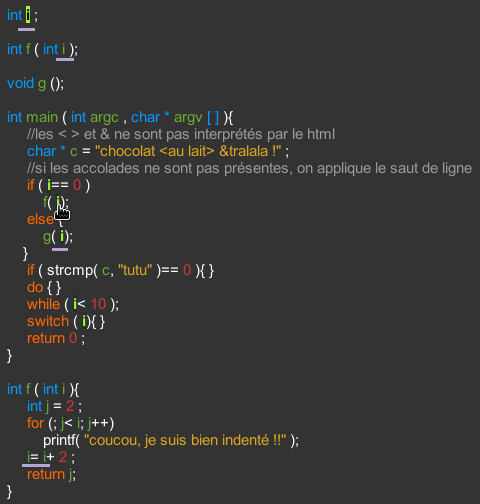
\includegraphics[height=10cm]{site/survol.png} 
	\newline
\textit{Mise en valeur des occurrences d'une variable au survol, avec distinction de la déclaration}
\newline 
ma solution est partielle, car cette manipulation permet de placer un identifiant avec le surnom de chaque fonction sur sa ligne de déclaration. Cependant, pour avoir un lien vers les déclarations de variables, je place aussi des balises supplémentaires qui peuvent faire doublons sur les fonctions. Je n'ai pas encore trouvée de solution pour éviter ce doublon et donc avoir un code html cohérent, bien que mes liens soient fonctionnels actuellement. \newline

\subsubsection*{afficher ou cacher les accolades}
Le contenu des accolades peut être caché ou affiché en cliquant sur les accolades ouvrantes. \newline
C'est implémenté avec une simple fonction java-script. \newline
Cette fonctionnalité n'a pas posée de réels problème, excepté lorsque j'ai voulue numéroter les lignes en utilisant uniquement le css. les balises code qui devaient encadrées chaque ligne entraient en conflit avec la balise span qui encadre le contenu des accolades. Cela aurait été résolu en plaçant la balise span a l'extérieur des balises de code qui encadrent la ligne où se trouve l'accolade ouvrante.
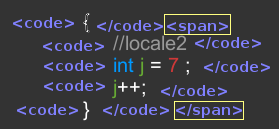
\includegraphics[height=10cm]{site/numerote.png} 
\textit{la structure des balises si j'avais pu mettre les numérotations}

\section{Partie Doxygen}

Les commentaires Doxygen servent à documenter un fichier C. La documentation est générée sous forme html. Elle a pour syntaxe :
\begin{verbatim}
/** (ou /!*)
 * \commande texte
 * \commande texte
 * texte
 * \commande texte
 */
\end{verbatim}

Les commandes Doxygen reconnues par notre projet sont : fn, brief, param et return. Une commande et son texte peuvent prendre une ou plusieurs ligne comme dans l'exemple ci-dessus.

La documentation est analysée, puis elle est générée en syntaxe html avec le css adéquat.

\subsection{Problèmes rencontrés}
Nous avons eu des problèmes sur la manière de reconnaître les différents motifs dans un commentaire doxygen car il n'y avait pas une ligne pour une commande. Finalement nous avons crée une "commande actuelle" qui se met à joue seulement quand il y a une nouvelle commande de lue.


\subsection{Améliorations possibles}
Une amélioration possible serait que l'analyseur récupère toutes les prototypes de fonction dans le .h et qu'il génère un début de commentaire doxygen avec les bonnes balises en fonction du nombre de paramètres de la fonction. L'utilisateur n'aurait plus qu'à rajouter son texte.

Une autre amélioration serait de gérer les balises-liens entres les descriptions de fonctions afin de faciliter le déplacement et la lecture de la documentation par l'utilisateur.

\end{document}
